\documentclass[]{pkuai4m}

% single-column: \documentclass[]{pkuai4m}, 
%Please prioritize using single-column。

% twocolumn: \documentclass[twocolumn]pkuai4m}

\usepackage[toc,page,header]{appendix}
\usepackage[UTF8]{ctex} % 增加中文支持

%%%%%%%%%%%%%%%%%%%%%%%%%%%%%%%%%%%%

\usepackage{minitoc}
\usepackage{multirow}     % 支持 \multirow
\usepackage{multicol}     % 支持多列排版（部分场景）
\usepackage{booktabs}     % \toprule \midrule \bottomrule
\usepackage{colortbl}     % 单元格或行着色
\usepackage[table]{xcolor} % 颜色支持（含 table 选项）
\usepackage{makecell}     % 允许在表格中换行 / 对齐
\usepackage{graphicx}     % 支持 \resizebox
% \usepackage{algorithm}
% \usepackage{algpseudocode}
\usepackage{minted}
\usepackage{xcolor}
\usepackage{fontawesome5}
\usepackage{svg}
\usepackage{caption}      % 用来给Archon图例排版
% \usepackage{listings}
% \usepackage{spverbatim}
\usepackage{fancyvrb}
\usepackage{fvextra}
\usepackage{enumitem}
\usepackage{wrapfig}
\usepackage{mathtools}

\setlength{\columnsep}{1.2em}

\usepackage[most]{tcolorbox}
\usepackage{amsthm,amsmath,amssymb}

\theoremstyle{plain}
\newtheorem{theorem}{定理}
\newtheorem{corollary}[theorem]{推论}
\newtheorem{lemma}[theorem]{引理}
\newtheorem{cited}[theorem]{引用结果}
\newtheorem*{theorem*}{定理}
\newtheorem*{problem*}{问题}

\theoremstyle{definition}
\newtheorem{definition}[theorem]{定义}
\newtheorem{notation}[theorem]{记号}
\newtheorem{remark}[theorem]{注记}
\newtheorem{problem}[theorem]{问题}

% \tcolorboxenvironment{theorem}{colback=blue!5, colframe=blue!50!black, fonttitle=\bfseries, sharp corners}
\tcolorboxenvironment{theorem}{
    colback=blue!5,           % 浅蓝色背景 (5% 蓝色)
    colframe=blue!5,          % 边框颜色与背景相同 → 无可见边框
    arc=1mm,                  % 圆角半径 (3mm，稍带圆角)
    fonttitle=\bfseries,      % 标题粗体
    boxrule=0pt,              % 边框线宽为0 (彻底去掉边框)
}
\tcolorboxenvironment{lemma}{
    colback=blue!5,           % 浅蓝色背景 (5% 蓝色)
    colframe=blue!5,          % 边框颜色与背景相同 → 无可见边框
    arc=1mm,                  % 圆角半径 (3mm，稍带圆角)
    fonttitle=\bfseries,      % 标题粗体
    boxrule=0pt,              % 边框线宽为0 (彻底去掉边框)
}
\tcolorboxenvironment{corollary}{
    colback=blue!5,           % 浅蓝色背景 (5% 蓝色)
    colframe=blue!5,          % 边框颜色与背景相同 → 无可见边框
    arc=1mm,                  % 圆角半径 (3mm，稍带圆角)
    fonttitle=\bfseries,      % 标题粗体
    boxrule=0pt,              % 边框线宽为0 (彻底去掉边框)
}
\tcolorboxenvironment{definition}{
    colback=red!5,           % 浅蓝色背景 (5% 蓝色)
    colframe=red!5,          % 边框颜色与背景相同 → 无可见边框
    arc=1mm,                  % 圆角半径 (3mm，稍带圆角)
    fonttitle=\bfseries,      % 标题粗体
    boxrule=0pt,              % 边框线宽为0 (彻底去掉边框)
}
\tcolorboxenvironment{problem*}{
    colback=orange!5,           % 浅蓝色背景 (5% 蓝色)
    colframe=orange!5,          % 边框颜色与背景相同 → 无可见边框
    arc=1mm,                  % 圆角半径 (3mm，稍带圆角)
    fonttitle=\bfseries,      % 标题粗体
    boxrule=0pt,              % 边框线宽为0 (彻底去掉边框)
}
\tcolorboxenvironment{cited}{
    colback=green!5,           % 浅蓝色背景 (5% 蓝色)
    colframe=green!5,          % 边框颜色与背景相同 → 无可见边框
    arc=1mm,                  % 圆角半径 (3mm，稍带圆角)
    fonttitle=\bfseries,      % 标题粗体
    boxrule=0pt,              % 边框线宽为0 (彻底去掉边框)
}
% \tcolorboxenvironment{lemma}{colback=green!5, colframe=green!50!black, sharp corners}
% \tcolorboxenvironment{corollary}{colback=purple!5, colframe=purple!50!black, sharp corners}
% \tcolorboxenvironment{definition}{colback=red!5, colframe=red!50!black, sharp corners}
% \tcolorboxenvironment{remark}{colback=yellow!5, colframe=yellow!50!black, sharp corners}
% \tcolorboxenvironment{problem*}{colback=red!5, colframe=orange!50!black, sharp corners}
% \tcolorboxenvironment{notation}{colback=gray!5, colframe=gray!50!black, sharp corners}




%%%%%%%%%%%%%%%%%%%%

\title{通过形式化验证实现自动猜想解决}

\author[1,5,\dagger,*]{Haocheng Ju}
\author[1,5,\ddagger,*]{Guoxiong Gao}
\author[2,*]{Jiedong Jiang}
\author[4,10,*]{Bin Wu}
\author[1,3,*]{Zeming Sun}
\author[1,5,10]{Leheng Chen}
\author[1,5]{Yutong Wang}
\author[1]{Yuefeng Wang}
\author[1,5]{Zichen Wang}
\author[1,5]{Wanyi He}
\author[5]{Peihao Wu}
\author[6]{Liang Xiao}
\author[6]{Ruochuan Liu}
\author[5,\P]{Bryan Dai}
\author[7,8,9,10\P]{Bin Dong}

\affiliation[]{
$^{1}$北京大学数学科学学院 \\
$^{2}$西湖大学理论科学研究院 \\
$^{3}$京都大学数理解析研究所 \\
$^{4}$天津大学数学学院 \\
$^{5}$IQuest Research \\
$^{6}$北京大学数学科学学院，新基石科学实验室 \\
$^{7}$北京大学北京国际数学研究中心及新基石科学实验室 \\
$^{8}$北京大学机器学习研究中心\\
$^{9}$大湾区大学（筹）智能计算中心 \\
$^{10}$中关村研究院 \\
}

\contribution[*]{共同第一作者}
\contribution[\dagger]{非形式智能体负责人}
\contribution[\ddagger]{形式化智能体负责人}
\contribution[\P]{通讯作者}




\abstract{
近年来，大型语言模型（LLM）的进步显著提升了它们进行数学推理的能力，从解决初等问题扩展到在研究级问题上表现出越来越强的能力。然而，由于自然语言推理固有的模糊性以及对严格验证的需求，可靠地解决和验证此类问题仍然具有挑战性。在本文中，我们提出了一种用于解决研究级数学问题的自动化框架，该框架将自然语言推理与形式化验证相结合，从而在极少的人工干预下实现端到端的问题求解。我们的框架包含两个组件：非形式推理智能体 Rethlas 和形式化验证智能体 Archon。Rethlas 通过将推理原语与我们的数学定理搜索引擎 Matlas 相结合，来模仿人类数学家的工作流程，以探索求解策略并构建候选证明。配备了我们的形式化定理搜索引擎 LeanSearch 的 Archon，通过结构化的任务分解、迭代改进和自动证明合成，将非形式论证转化为完全形式化的 Lean 4 项目，从而确保机器可检查的正确性。使用该框架，我们自动解决了一个由 D. D. Anderson (2014) 提出的交换代数中的开放问题，并在几乎没有人类参与的情况下在 Lean 4 中对生成的证明进行了形式化验证。我们的实验表明，强大的定理检索工具能够发现和应用深刻的跨领域数学技术，而形式化智能体能够自主填补非形式论证中非平凡的空白。更广泛地说，我们的工作说明了一种有前景的数学研究范式，在这种范式中，配备定理检索工具的非形式和形式推理系统协同运作以产生可验证的结果，大幅减少人力，并提供了人类-AI 协同数学研究的具体实例。
}

\date{\today}
% \correspondence{Author1 at \email{xxx@pku.edu.com}, Author5 at \email{xxx}}



\def\emailicon{\raisebox{-1.5pt}{
\includegraphics[height=1.05em]{pkuai4m/email_logo.pdf}}}
\def\githubicon{\raisebox{-1.5pt}{
\includegraphics[height=1.05em]{pkuai4m/github_logo.pdf}}}
\def\huggingfaceicon{\raisebox{-1.5pt}{
\includegraphics[height=1.05em]{pkuai4m/huggingface_logo.pdf}}}
\def\platformicon{\raisebox{-1.5pt}{
\includegraphics[height=1.05em]{pkuai4m/matlas_logo.png}}}

% * Equal Contribution \quad $\dagger$ Project Leader \quad $\ddagger$ Corresponding author

% \contribution[*]{Equal Contribution}
% \contribution[\dagger]{Project Leader}
% \contribution[\ddagger]{Corresponding author}


\checkdata[ \emailicon \hspace{0.3em} Correspondence ]{\email{cbdai@iquestlab.com}, \email{dongbin@math.pku.edu.cn}}

% % define linking
\newcommand{\rethlaslink}{https://github.com/frenzymath/Rethlas}
\newcommand{\archonlink}{https://github.com/frenzymath/Archon}
 \newcommand{\resultslink}{https://github.com/frenzymath/Anderson-Conjecture}
 
% \newcommand{\datalink}{https://huggingface.co/FrenzyMath/matlas}
 %\newcommand{\platformlink}{https://matlas.ai/}

% % You can add additional info fields as follows 
  \checkdata[ \githubicon \hspace{0.3em} Rethlas Source]{ \url{\rethlaslink} }
    \checkdata[ \githubicon \hspace{0.3em} Archon Source]{ \url{\archonlink} }
 \checkdata[ \githubicon \hspace{0.3em} Formalization Results ]{ \url{\resultslink} }

%\checkdata[ \huggingfaceicon \hspace{0.3em} Dataset ]{ \url{\datalink} }
%\checkdata[ \platformicon \hspace{0.3em} Web service ]{ \url{\platformlink} }





\begin{document}
\maketitle

% footnote
\renewcommand{\thefootnote}{\fnsymbol{footnote}} 
\setcounter{footnote}{0}

% 

\renewcommand{\thefootnote}{\arabic{footnote}}
\pagestyle{fancy}
\fancyhf{}
\fancyhead[R]{\thepage}

% Content
%\newpage
%\tableofcontents
%\newpage

\section{引言}

近年来，大型语言模型（LLM）的数学推理能力发展迅速，从处理初等算术和高中级别问题，发展到在本科课程中表现出胜任力，并开始参与研究生和研究级别的数学问题。早期的模型（如 GPT-3）在基本算术上都遇到了困难，而 GPT-4 \cite{achiam2023gpt} 在小学级别的基准测试 GSM8K 上取得了很高的分数（92\%）。随着\textit{测试时计算扩展（test-time scaling）}的出现，模型在推理期间分配更多的计算资源用于推理，诸如 OpenAI 的 o1 等系统在包括 AIME 在内的高中竞赛问题上表现出了强大的性能。随后的推理模型 \cite{guo2025deepseek,qwq32b,yang2025qwen3,comanici2025gemini} 进一步验证了这一范式的有效性。Google 的 Gemini Deep Think 实现了一个显著的里程碑，它完全使用自然语言推理在国际数学奥林匹克（IMO）中达到了金牌级别的表现。

在更高的层面上，最近的研究表明，LLM 在本科和研究生数学方面也变得越来越有能力，同时在研究级问题上继续取得进展。例如，\cite{ju2026ai} 表明，当时可用的前沿模型，如 Gemini 2.5 Pro，在本科数学考试基准测试中得分超过 90 分。同一项研究还发现，o3-mini 在分析、概率、代数和几何与拓扑的博士资格考试中平均得分超过 80 分。开源模型也表现出了强劲的性能；例如，\cite{jiang2025fate} 报告称 DeepSeek-R1 在研究生级代数任务上实现了 71.0\% 的证明准确率。在研究级别，进展正在进行中。在 \textit{FrontierMath} 基准测试 \cite{glazer2024frontiermath}（其 Tier 4 包含未发表的研究级问题）上，o3-mini 仅达到 4\% 的 pass@1 准确率，而 GPT-5 将其提高到 15\%。最近，领先的系统 GPT-5.4-Pro (web) 达到了 38\% 的 pass@1 准确率。值得注意的是，GPT-5.4-Pro 还解决了一个来自 \textit{FrontierMath} 组合数学中被归类为“中等有趣”的开放问题。基于这些前沿模型，配备适当治理工程的基于 LLM 的智能体可以进一步提高性能。例如，\textit{Aletheia} 智能体 \cite{feng2026towards} 整合了生成器、验证器和修订器，已经自主处理了四个 Erdős 问题 \cite{feng2026semi}，并解决了诸如计算算术 Hirzebruch 比例原理的特征权重 \cite{feng2026eigenweights} 以及关于 Hodge 丛简单性的问题 \cite{patel2026simplicity} 等研究问题。

然而，尽管取得了这些进展，评估 LLM 和基于 LLM 的智能体的研究级能力仍然是一个需要大量人力的重大瓶颈。随着数学复杂性的增加，评估越来越依赖于领域专家；然而，由于自然语言固有的不精确性，即使是经验丰富的数学家有时也会误判论证。事实上，即使在顶级期刊严格的同行评审过程中，错误也可能持续存在。为了实现快速可靠的数学推理验证，因此有必要转向更加机械化和无歧义的框架。形式化系统恰好提供了这样一个基础。形式化系统提供了一种精确的符号语言，配以严格定义的构建和验证证明的机制。一旦数学论证在保留其语义内容的同时被翻译成形式语言，其正确性就可以以完全的严谨性得到验证。

受此启发，我们提出了一种用于自主处理和验证研究级数学问题的框架，该框架将自然语言推理智能体与形式化智能体集成在一起，从而在极少的人工监督下实现端到端的问题解决。非形式智能体 Rethlas\footnote{Rethlas 在 \href{https://github.com/frenzymath/Rethlas}{https://github.com/frenzymath/Rethlas} 开源。}，旨在模仿人类数学家的工作流程，并配备了定理检索等工具来探索候选解决方案路径。形式化智能体 Archon \footnote{Archon 在 \href{https://github.com/frenzymath/Archon}{https://github.com/frenzymath/Archon} 开源。} 建立在双智能体、工具增强的架构之上，并配备了我们的形式化定理搜索引擎 LeanSearch \cite{gao2024semantic}。它通过结构化规划、迭代形式化和持久的内存管理将非形式证明转化为完全验证的 Lean 4 项目，从而确保正确性和可扩展性。

使用该框架，我们自动解决了一个由 D. D. Anderson 在 2014 年提出的交换代数开放问题 \cite{cahen2014open}，并在几乎没有人工干预的情况下在 Lean 4 中对生成的证明进行了形式化验证。在自然语言求解阶段，Rethlas 采用的语义定理搜索引擎 Matlas 在发现 Jensen \cite{jensen2006completions} 的一个关键技术结果方面发挥了至关重要的作用。在形式化过程中，Archon 通过填补参考文献和自然语言证明中留下的非平凡空白，展示了其强大的数学能力。形式化已经通过了 Comparator\footnote{https://github.com/leanprover/comparator} 的检查。

本文的其余部分结构如下。在\Cref{sec:related}中，我们回顾了关于自然语言和形式推理智能体的相关工作。\Cref{sec:overview}提供了我们框架的概述。用于非形式证明生成的实验结果呈现在\Cref{sec:rethlas_results}中，而形式化结果在\Cref{sec:archon_results}中讨论。最后，\Cref{sec:concl}对全文进行总结。

\section{相关工作}\label{sec:related}
\subsection{用于自然语言推理的智能体}

基于 LLM 的智能体最近在高中奥林匹克数学和研究级数学中都表现出了强劲的性能。在奥林匹克数学方面，一项代表性的工作是 \cite{huang2025winning}，它提出了一种验证和改进的流水线，使用 Gemini 2.5 Pro、Grok-4 和 GPT-5 等模型成功解决了 2025 年 IMO 的 6 道题中的 5 道。这显著超越了这些模型在没有这种结构化工作流程下的基线性能。

在研究级别上，\textit{Aletheia} 智能体 \cite{feng2026towards} 建立在 Gemini Deep Think 的高级版本之上，通过涉及生成器、验证器和修订器的迭代过程进行操作。它以自主方式处理了四个 Erdős 问题 \cite{feng2026semi}，并在人机协作的半自主设置下处理了一个广义 Erdős 问题 \cite{barreto2026irrationality}。除此之外，\textit{Aletheia} 还解决了一些真正的研究问题，包括计算算术 Hirzebruch 比例原理的特征权重 \cite{feng2026eigenweights} 和建立独立集的界限 \cite{lee2026lower}。此外，\textit{Aletheia} 解决了 FirstProof 基准测试 \cite{feng2026aletheia}（在 \cite{abouzaid2026first} 中引入）中 10 个问题里的 6 个，该基准测试由人类数学家解决但在评估时尚未公开发布的真实研究问题组成。与此同时，\textit{FullProof} 系统 \cite{bryan2026motivic} 展示了代数几何中有效的人机协作：AI 处理特殊情况，人类提供一般情况的见解，然后 AI 根据这些提示完成一般解决方案。

\subsection{用于形式推理的智能体}

针对 Lean 4 的几个智能体系统最近在竞赛级基准测试中取得了优异成绩。AlphaProof~\cite{hubert2025olympiad}，来自 Google DeepMind 的首创基于 RL 的智能体，在 2024 年 IMO 取得了银牌表现。Seed-Prover 1.5~\cite{chen2025seed} 将工具调用能力直接训练到模型中，解决了 2025 年 Putnam 的 12 道题中的 11 道。AxiomProver~\cite{breen2025ax} 和开源的 Numina-Lean-Agent~\cite{liu2026numina} 分别解决了所有 12 道题。Harmonic 的 Aristotle~\cite{achim2025aristotle} 用 MCTS 和非形式推理流水线增强了微调的证明搜索模型，达到了 2025 年 IMO 金牌表现，并为社区提供了公共 API。

超越竞赛基准测试，这些系统中的几个已经展示了研究级能力。Aristotle 和 AxiomProver 都在 Lean 中形式化了开放 Erd\H{o}s 问题的解答；AxiomProver 还解决并形式化了诸如关于数值半群的合冲的 Fel 猜想~\cite{chen2026fel} 等开放研究猜想。在更多人类参与下，Numina-Lean-Agent 与两位人类专家协作形式化了 Brascamp--Lieb 定理~\cite{liu2026numina}，而 VML 项目~\cite{ilin2026semi} 在一位数学家十天的交互式指导下形式化了数学物理中的一个结果。在更大规模上，Math, Inc. 的 Gauss~\cite{mathinc_spherepacking} 生成了大约 200,000 行 Lean 代码来形式化验证获得菲尔兹奖的球堆积证明；对于 8 维，Gauss 建立在人类准备的蓝图的预先存在的代码库上，而 24 维则从原始论文中自动形式化。在工具方面，Mistral 的 Leanstral~\cite{mistralai2026leanstral} 提供了一个专为研究级形式化项目中的证明工程而设计的开源智能体。

\section{框架概述}\label{sec:overview}

\begin{figure}[tb]
\centering
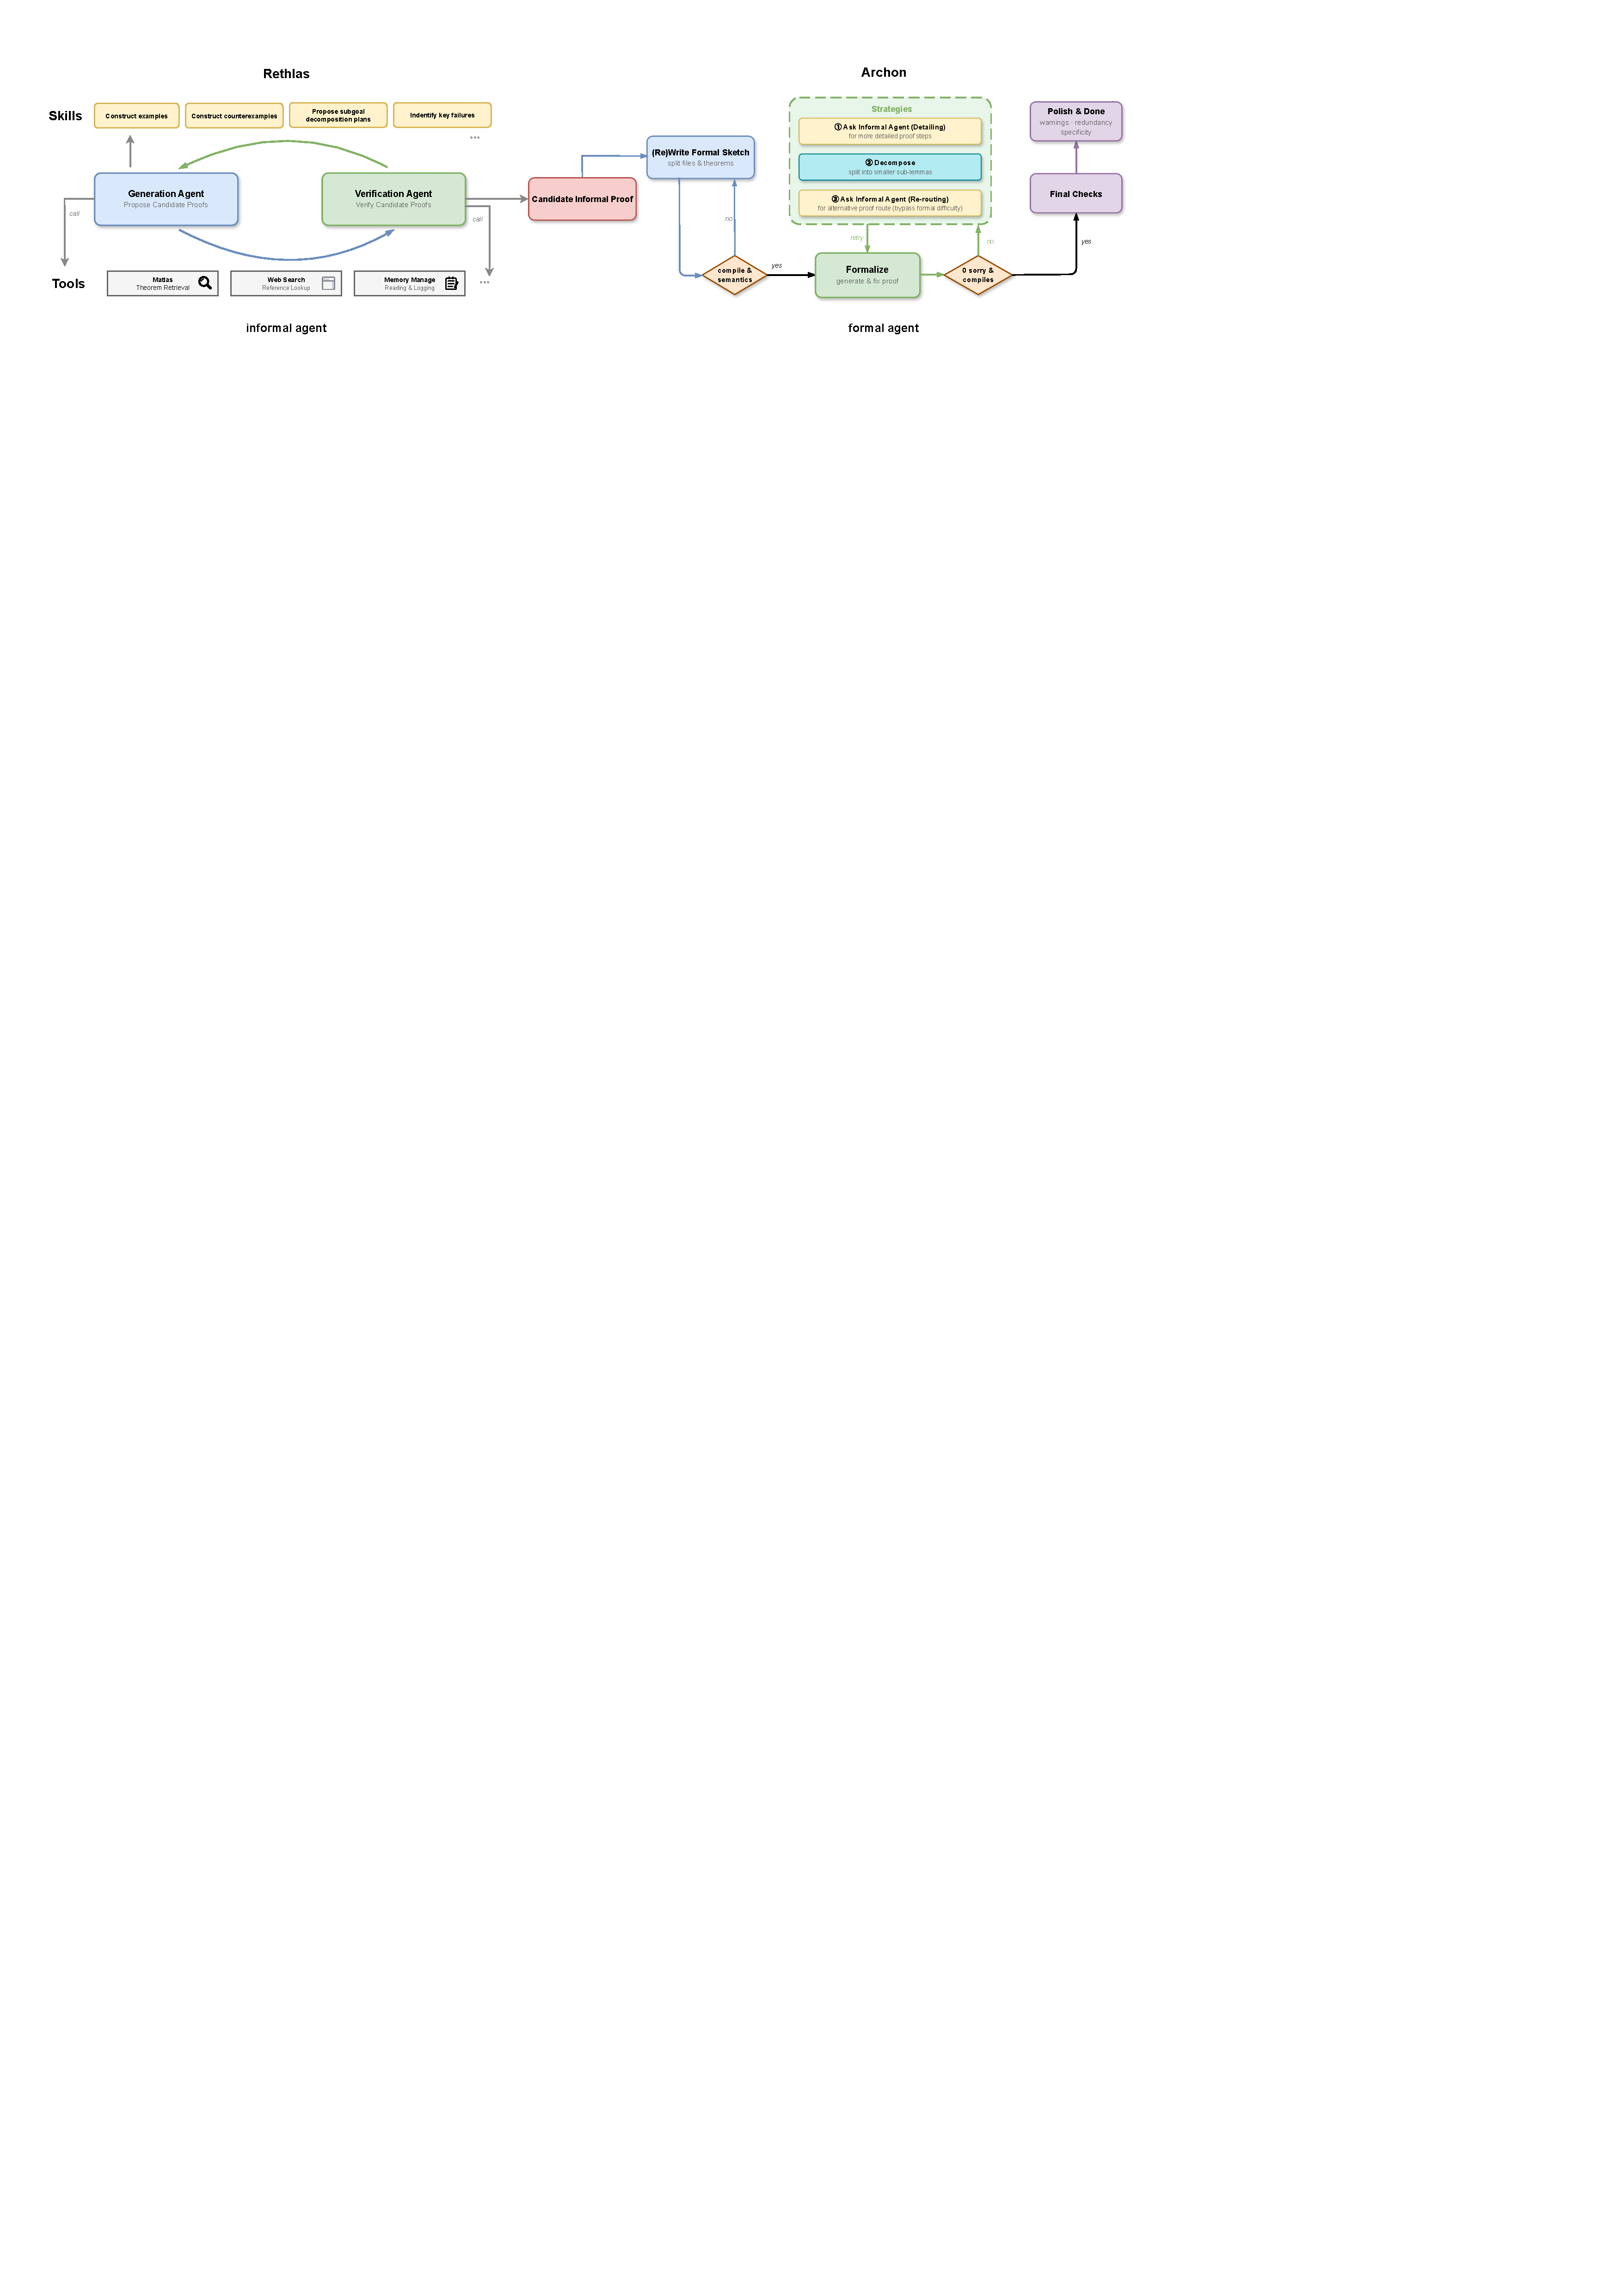
\includegraphics[width=0.99\linewidth]{figure/whole.pdf}
\caption{框架流程概述。}
\label{fig:complete}
\end{figure}




在本节中，我们描述了用于自主处理和验证研究级数学的框架。该框架包含一个非形式智能体（Rethlas），它首先生成一个潜在正确的候选证明，以及一个形式化智能体（Archon），它将这个非形式证明翻译成形式语言 Lean 4，并在形式化过程中填补任何空白（参见\Cref{fig:complete}）。非形式智能体 Rethlas 的设计呈现在\Cref{subsec:rethlas}中，而形式化智能体 Archon 的设计呈现在\Cref{subsec:archon}中。







\subsection{Rethlas：非形式智能体}\label{subsec:rethlas}








Rethlas 包含两个子智能体：生成智能体和验证智能体。如\Cref{fig:rethlas}所示，它在迭代过程中运行，其中生成智能体产生非形式证明并将其传递给验证智能体进行正确性检查。如果证明通过了验证，它被认为是一个候选非形式证明并且过程终止。否则，验证智能体会提供反馈，该反馈会传回生成智能体以修改证明。

\textbf{生成智能体。} 生成智能体旨在模仿人类数学家的工作流程，并配备了为数学研究量身定制的技能和工具。这些技能包含从数学家解决研究问题时采用的过程中提取的推理原语，它们包括：
\begin{itemize}
    \item \emph{构造玩具示例（toy examples）。} 当推理停滞不前并且需要更简单的实例来重新获得牵引力时使用此技能。构造的示例应该同时满足假设和结论，使人们能够观察假设如何生效并培养直觉。在应用此技能时，应该寻找示例中建议的重复模式、不变量或潜在的证明策略。推理、分解和检索也可用于识别合适的示例或简化设置。
    \item \emph{构造反例。} 当一个猜想或中间主张显得脆弱或不充分合理时使用此技能。目标是测试假设是否成立而结论失败。在应用此技能时，应利用推理、分解和检索来识别标准的障碍、病态构造或已知反例。
    \item \emph{搜索相关结果。} 此技能用于获取与当前问题相关的定理、构造、示例、反例或背景知识。它在构造示例或反例时，或者在证明需要支持性参考的子目标时也很有用。当发现可能有用的定理时，应使用来源的周围上下文展开所涉及的定义和概念，仔细验证其对当前设置的适用性，并明确不同上下文之间术语的任何变化。此外，不应仅停留在陈述本身，还应检查证明以提取有用的技术、构造、归约或证明模式。
    \item \emph{提出子目标分解计划。} 在从示例、反例、搜索结果和先前的尝试中收集到足够的见解后使用此技能。
    \item \emph{直接证明。} 一旦有一个或多个分解计划可用，就应用此技能。通过尝试直接证明其子目标来评估每个计划，同时在计划未完全成功时识别关键障碍。
    \item \emph{递归证明。} 当所有当前的分解计划都通过直接证明尝试过但没有一个完全成功时使用此技能。在这种情况下，会并行部署多个子智能体，每个子智能体分配一个分解计划以及与其相关的关键困难和其他计划中发现的困难。每个子智能体可以细化、扩展或局部修改其分配的计划，同时保持连续性而不是完全丢弃它。
    \item \emph{识别关键失败。} 当跨所有分解计划的递归尝试均失败时使用此技能。目标是识别这些失败中的常见模式，例如反复出现的障碍、无效的分解策略或缺失的背景知识。然后总结这些见解以指导下一轮计划生成。
\end{itemize}






\begin{figure}[tb]
\centering
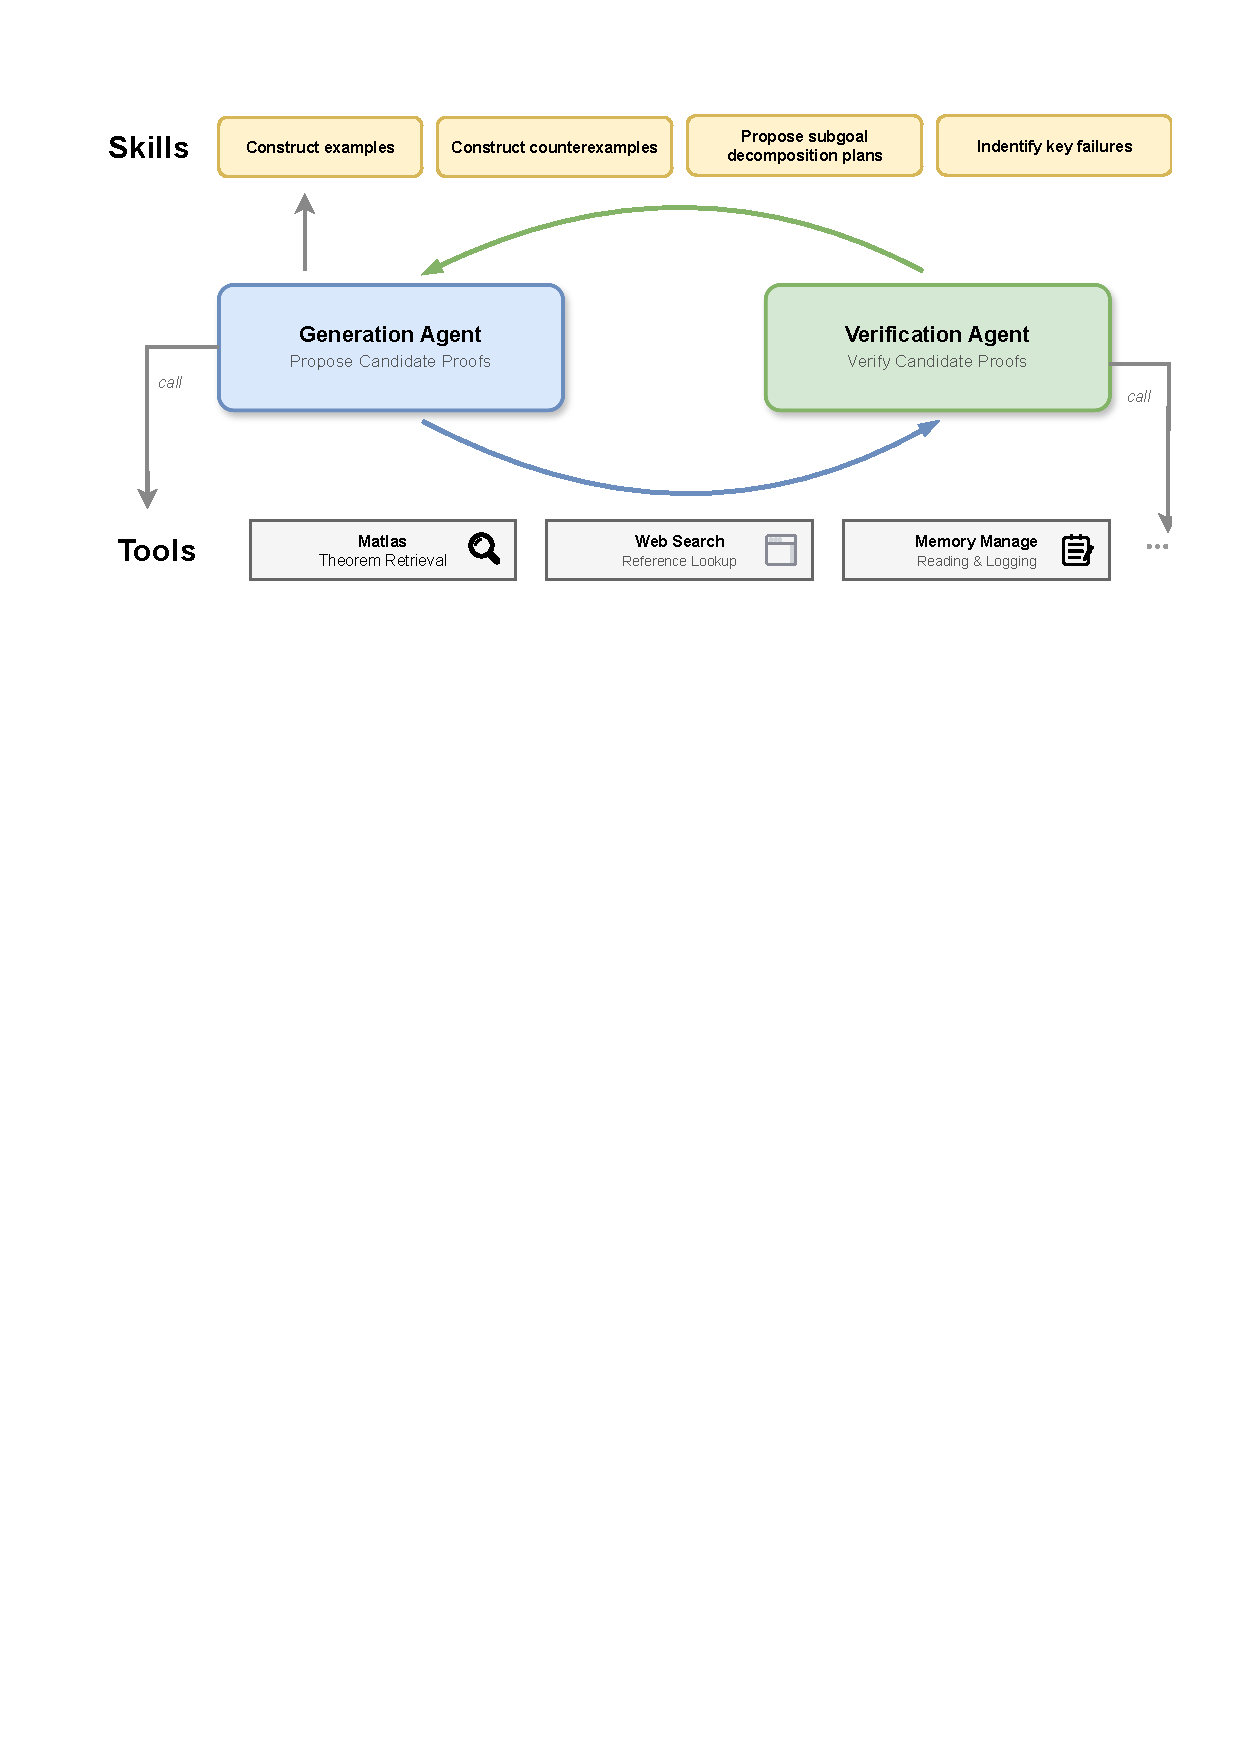
\includegraphics[width=0.6\linewidth]{figure/rethlas.pdf}
\caption{Rethlas 智能体。}
\label{fig:rethlas}
\end{figure}






正如上述描述所反映的那样，这些技能并不是孤立的，而是相互关联的。应用一项技能通常涉及其他技能的元素。例如，构造示例和反例并不是孤立发生的；它通常需要推理、问题分解和检索来识别适当的构造。在处理数学问题时，智能体被指示评估当前状态并选择要应用的适当技能，而不是事先决定固定的技能顺序。

在 Rethlas 使用的工具中，我们的定理搜索引擎 Matlas \footnote{Rethlas 实验中使用的 Matlas 版本是一个初步的内部测试系统，作为一个基于 arXiv 的定理搜索引擎，位于 \href{https://leansearch.net/thm/}{https://leansearch.net/thm/}。其语料库包含大约 1360 万条直接从 arXiv 论文中提取而未进一步处理的数学陈述。我们最新的 Matlas 系统，位于 \href{https://matlas.ai/}{https://matlas.ai/}，是一个更高级的定理搜索引擎，建立在从 180 种期刊和 1900 多本教科书的 435K 篇已发表论文中收集的 851 万条陈述之上。因此，它提供了更可靠和精选的数学结果来源。此外，我们提取陈述依赖关系并执行层次展开以使陈述更加自包含，这与早期基于 arXiv 的版本相比进一步提高了它们的可用性和质量。之前基于 arXiv 的定理搜索引擎将在不久的将来被弃用。} 发挥着核心作用。在我们的实验中，Matlas 作为一个针对 arXiv 数学陈述（包括定义、命题、定理、推论、示例和注记）的语义搜索引擎。其语料库包含大约 1360 万条这样的陈述，每条都嵌入到一个向量数据库中。给定一个数学陈述形式的查询，Matlas 嵌入查询并使用余弦相似度执行最近邻搜索以检索相关结果。与一般网络搜索相比，Matlas 提供了一种更细粒度且有原则的针对数学内容的检索机制。虽然其语料库较小，但它更加结构化，并能够更精确地识别相关陈述。在应用 \texttt{search-math-results} 技能时，Rethlas 被指示首先查询 Matlas 并检索相关的定理、示例或反例。然后它可以随后使用网络搜索要么跟进并查找原始论文进行详细检查，要么在 Matlas 结果不够用时补充搜索结果。

此外，Rethlas 维护一个工作内存，记录在推理过程中生成的中间工件，例如构造的示例、反例和子目标分解计划。智能体被指示将这些工件写入内存，并在需要时查询此内存，从而实现对先前生成见解的重用，并提高跨推理步骤的连贯性。在我们的实验中，生成智能体是使用 OpenAI Codex 智能体框架实现的，以 GPT-5.4 作为基础模型。

\textbf{验证智能体。} 验证智能体配备了检查数学证明正确性的技能。这些包括顺序验证陈述，例如检查跳过或含糊的步骤，识别关键错误和漏洞，以及仔细评估表面上未使用的假设是否真的多余，或者相反表明论证有遗漏。它们还包括确认引用的陈述，通过使用我们的定理搜索工具 Matlas 和网络搜索，检查被引用的陈述是否存在且适用于当前上下文，使用源论文的上下文扩展引用的陈述中的定义和术语，并确保当前证明中使用的术语与被引用来源中的术语具有相同的含义，因为相同的词语在不同的上下文中可能具有不同的定义。在我们的实验中，验证智能体是使用 OpenAI Codex 智能体以 GPT-5.4 作为底层模型实现的。

\subsection{Archon：形式化智能体}\label{subsec:archon}

数学证明要求完全的严谨性，然而即使是专家撰写的证明也可能包含细微的缺陷，而 LLM 产生的证明更容易出现幻觉，其可靠性要低得多。为了获得值得信赖的正确性保证，我们在流程中引入了形式化验证。如果证明通过了形式化语言编译器，那么验证正确性就归结为检查顶层陈述及其支持性定义是否忠实地捕捉了预期的数学内容。

我们采用 Lean 4 作为我们的形式化语言。其社区维护的库 Mathlib 包含由 770 多名成员贡献的超过 267,000 个定理和 127,000 个定义，提供了一个成熟的基础，使得前沿数学的形式化变得可行，因为每个依赖的定义和引理最终都必须建立在现有库的基础上。

形式化智能体 \textit{Archon} 扩展了我们之前关于陈述自动形式化的工作~\cite{gao2024herald, wang2025aria}，使其能够进行完整的证明形式化：给定一个非形式证明，它生成一个 Lean 4 项目，陈述并证明目标定理及其所有支持性定义和引理，且均基于 Mathlib。
Archon 首先通过收集依赖的参考文献来初始化项目，然后形式化关键的陈述和定义，将它们组织到特定主题的文件中。它通过迭代地填补文献中省略的空白，在遇到困难时咨询非形式智能体或外部来源，并探索替代的形式化策略，直到整个项目成功编译。

在将其部署到 Rethlas 生成的证明上之前，我们在 FirstProof~\cite{abouzaid2026first}（包含 10 个当时没有公开发布解决方案的研究级问题的集合，从而避免了数据污染）上验证了 Archon。OpenAI~\cite{openai_first_proof_2026} 和 Google~\cite{feng2026aletheia} 都在这些问题上评估了他们的系统。我们根据 Mathlib 的基础设施支持和数学意义选择了问题 4 和 6；值得注意的是，Google 的 Aletheia 在这两个问题上都失败了，而 OpenAI 成功了，但需要人工监督。Archon 为这两个问题的 OpenAI 非形式证明生成了完整的形式化：问题 6 是完全自主形式化的，而问题 4 仅在一个引理的证明倾向上需要一次自然语言提示。问题 4 的形式化大约耗时 50 小时，API 成本为 \$1,200；问题 6 耗时 30 小时，成本为 \$750。\footnote{有关更多详细信息，请参阅我们的博客文章 \url{https://frenzymath.com/blog/archon-firstproof/}}\Cref{subsubsec:workflow}回顾了工作流程和架构，而\Cref{subsubsec:enhancements}描述了自最初发布以来的增强功能。

\subsubsection{系统架构与工作流设计\label{subsubsec:workflow}}

\begin{figure}[!htbp]
    \centering
    \vspace{-0.6em}

    \begin{minipage}[t]{0.49\textwidth}
        \centering
        \vspace{0pt}
        \begin{minipage}[b][5.0cm][b]{\linewidth}
            \centering
            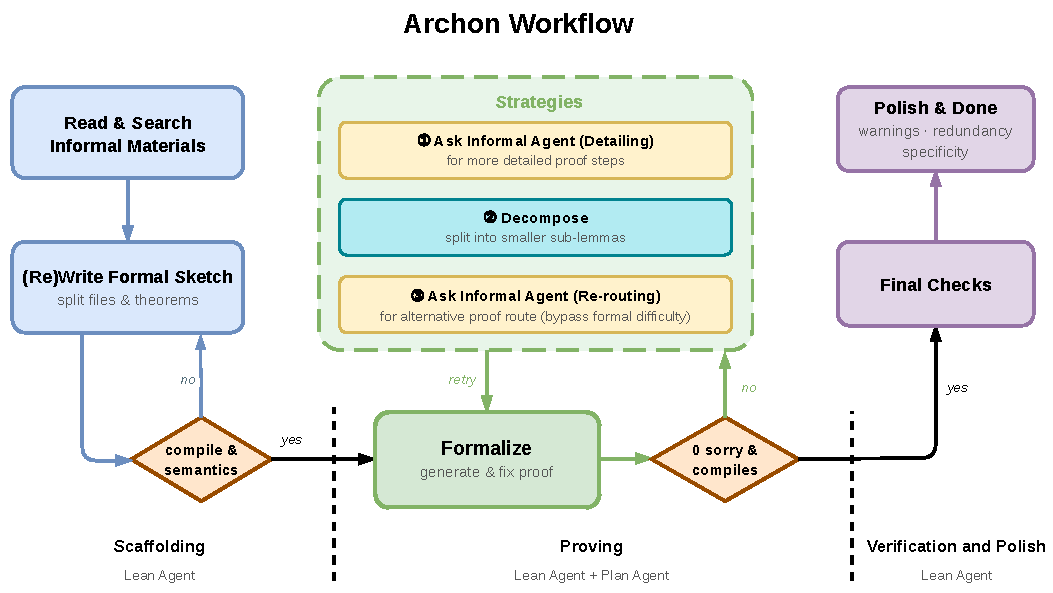
\includegraphics[
                width=\linewidth,
                height=5.0cm,
                keepaspectratio
            ]{figure/Archon_Workflow.pdf}
        \end{minipage}
        \vspace{-1.8em}
        \captionof{figure}{Archon 工作流}
        \label{fig:archon-workflow}
    \end{minipage}\hspace{0.005\textwidth}%
    \begin{minipage}[t]{0.49\textwidth}
        \centering
        \vspace{0pt}
        \begin{minipage}[b][5.0cm][b]{\linewidth}
            \centering
            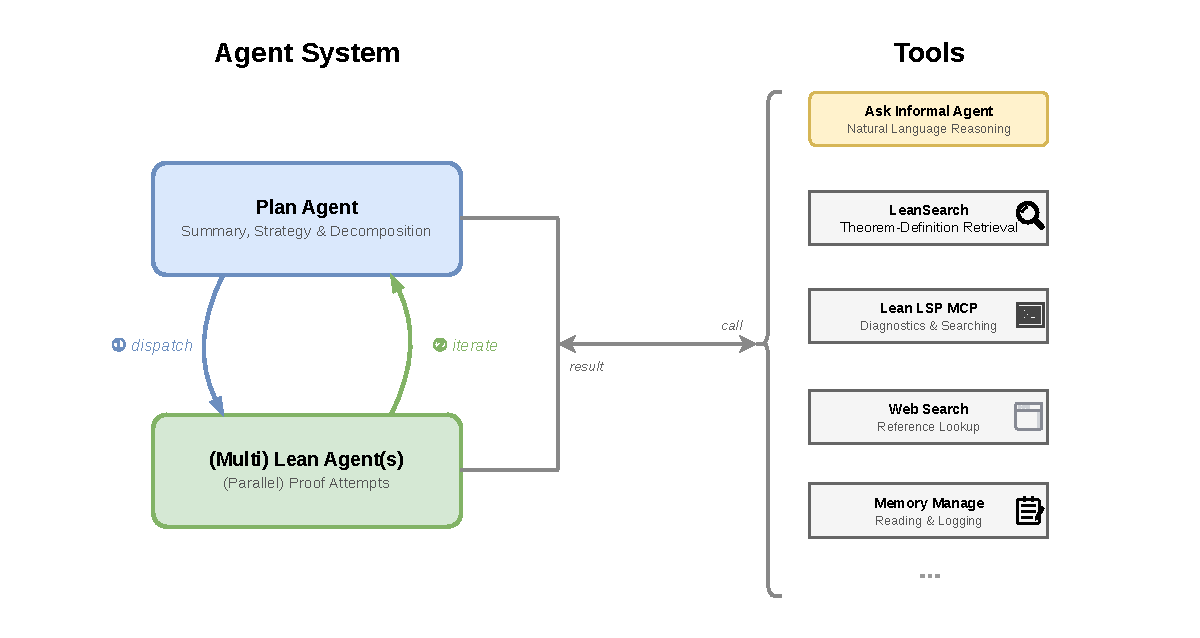
\includegraphics[
                width=\linewidth,
                height=5.0cm,
                keepaspectratio
            ]{figure/Agent_system_with_tools.pdf}
        \end{minipage}
        \vspace{-1.8em}
        \captionof{figure}{智能体系统与工具}
        \label{fig:agent-system-tools}
    \end{minipage}

    \vspace{-0.6em}
\end{figure}

我们的核心设计原则是避免硬编码的工作流，而是为智能体配备足够的技能和工具，赋予其最大的自主权。然而，我们观察到在长时间运行的会话中，特别是当智能体面临困难的引理时，累积的上下文会降低性能：智能体自身的失败尝试和悲观注释会削弱其坚持下去的意愿。为了解决这个问题，我们引入了一种双智能体架构，包括一个\textbf{规划智能体（Plan Agent）}（在一个全新的上下文中运行，用于分解任务并提供针对性的指导）和一个\textbf{Lean 智能体（Lean Agent）}（在一个受限的范围内执行形式化）。这种分离显著减轻了上下文污染和任务厌恶（例如，包含累积失败的上下文被观察到与智能体在困难义务上的坚持度降低相关）。

形式化过程分为三个阶段（\Cref{fig:archon-workflow}）：
\begin{enumerate}
    \item \textbf{搭建脚手架（Scaffolding）。} Lean 智能体分析非形式证明并构建初始文件结构：将证明拆分为模块，定义定理签名，并在每个证明义务处放置 \texttt{sorry} 占位符。这种分解不是固定的，可能会随着证明的发展而修改。
    \item \textbf{证明（Proving）。} Lean 智能体和规划智能体进入一个迭代循环。Lean 智能体尝试消除 \texttt{sorry} 占位符；当遇到困难时，它会将诊断信息返回给规划智能体，规划智能体会重新评估证明策略并分发修改后的任务。当分解产生独立的证明义务时，多个 Lean 智能体可以并行运行。
    \item \textbf{验证和打磨（Verification and Polish）。} 系统确认成功编译，并且不存在 \texttt{sorry}、\texttt{axiom} 等逃生通道，然后执行质量检查以提取可重用的引理并降低证明复杂性。
\end{enumerate}

如\Cref{fig:agent-system-tools}所示，智能体配备了一套通过终端 CLI 和模型上下文协议（MCPs）实现的工具。我们强调两个对 Archon 有效性特别重要的工具：

\textbf{咨询非形式智能体。} 当 Lean 智能体需要超出所提供的非形式证明涵盖范围的数学指导时，它会委托给非形式智能体以获取自然语言的子证明或替代策略。在大多数情况下，这是一个轻量级的 Gemini API 调用以进行快速推理。当智能体遇到更实质性的障碍时，它可能会调用 Rethlas 进行更深入、长期限的推理。

\textbf{LeanSearch。} 我们之前发布并在 Lean 社区广泛采用的检索工具，提供了对 Mathlib 定理和定义的模糊搜索。对于 Archon，我们进一步提高了它的检索准确性，并将其更新到最新的 Lean 和 Mathlib 版本。至关重要的是，LeanSearch 使智能体能够可靠地确定 Mathlib 中是否已经存在所需的结果，从而允许它在何时调用库引理和何时从头开始形式化做出充分知情的决策。这种能力对于产生充分利用现有基础设施的形式化至关重要。

其他工具包括用于编译诊断的 Lean LSP MCP、用于检索已发表参考文献的 Web 搜索，以及一个内存管理系统，该系统在上下文压缩和会话重启之间持久保存智能体的架构推理、失败的方法和学习到的技术。

仅仅提供工具是不够的；模型还需要关于何时以及如何部署它们的明确指导。这种行为指导编码在\textbf{技能（skills）}中，这些技能是建立在 Lean 4 技能框架上的结构化指令文件，它们塑造了智能体的工作模式和边界情况处理，以反映真实的形式化实践。







\subsubsection{用于猜想形式化的增强功能\label{subsubsec:enhancements}}

用于 FirstProof 问题 4 和 6 的 Archon 版本验证了双智能体架构：规划智能体在很大程度上消除了 Lean 智能体停滞或拒绝推进的情况。然而，扩展到更难的问题揭示了两个进一步的挑战。首先，随着数学难度和项目复杂性的增长，智能体偶尔会忘记先前的尝试，反复探索相同的死胡同，浪费计算资源。其次，随着项目扩大，智能体必须管理不断增加的非形式参考资料体，并且在需要时可能难以找到它们。我们引入了两个已开源的增强功能来解决这些问题。

\textbf{内存系统和复查智能体（Review Agent）。} 我们缩短了每个 Lean-Plan 迭代的持续时间，并要求每个智能体记录其会话的摘要。跨会话维护了几个全局状态文档，跟踪总体工作流阶段、每个文件的证明状态，以及局部 \texttt{sorry} 消除和重构工作的详细记录。此外，一个\textbf{复查智能体}在每个会话边界运行，以综合最近会话的趋势。这种多会话视角对于检测停滞（仅表现为连续会话的模式）至关重要。虽然复查智能体不改变形式化本身，但它使规划智能体能够在正确的时间调整策略，并为人类专家提供更清晰的进度视图。

\textbf{结构化提示和参考文献管理。} 我们将智能体的指导和参考材料重新组织成清晰的目录结构。在项目初始化期间，人类专家（在智能体的协助下）准备论文参考资料，然后智能体通过搜索添加进一步的参考资料。在面临数学困难时，智能体咨询非形式智能体，然后将候选的证明路线记录在与原始参考资料截然不同的专用位置。控制智能体工作模式和约定的技能和提示可以按项目进行自定义；在我们的实验中，当非形式参考步骤被认为是可信的时，明确指示规划智能体遵循这些步骤，显著减少了在没有前途的替代方案上花费的时间。这种设计还保持了上下文的整洁：智能体仅加载与当前任务相关的材料，避免被无关信息分心。

\medskip
\noindent 这些设计选择在\Cref{sec:archon_results}中描述的全规模形式化中起着核心作用。

\section{开放问题及 Rethlas 的解答}\label{sec:rethlas_results}

框架建立后，我们现在将注意力转移到目标数学问题上。\Cref{subsec:open_problem}介绍了背景和 Anderson 的开放问题。\Cref{subsec:nl_proof_sketch}然后给出了 Rethlas 生成的证明的概述。最后，\Cref{subsec:discovery}追溯了产生证明的逐步发现过程。

\subsection{Anderson 的开放问题}\label{subsec:open_problem}


设 \((R, \mathfrak{m})\) 为诺特局部环。回顾以下定义：
\begin{enumerate}[leftmargin=*]
    \item $R$ 被称为是 \emph{拟完备的（quasi-complete）}，如果对于 $R$ 的理想的每一个递降序列 $\{A_n\}_{n\ge 1}$ 以及每一个整数 \(k \ge 1\)，存在 \(s_k\) 使得
    \[
    A_{s_k} \subseteq \Bigl(\bigcap_{n\ge 1} A_n\Bigr) + \mathfrak{m}^k.
    \]

    \item $R$ 被称为是 \emph{弱拟完备的（weakly quasi-complete）}，如果上述条件对于满足 \(\bigcap_{n \ge 1} A_n = 0\) 的所有递降序列都成立；在这种情况下，该条件简化为
  \[
  A_{s_k} \subseteq \mathfrak{m}^k.
  \]
\end{enumerate}

这些性质自然产生于对局部环拓扑的研究。拟完备显然蕴含弱拟完备，而每一个完备局部环都是拟完备的这一推论最初是由 Chevalley 证明的 \cite[Lemma 7]{chevalley1943theory}。D. D. Anderson 提出了以下问题：

\begin{problem*}[{D. D. Anderson, \cite[Problem 8a]{cahen2014open}}]
对于诺特局部环，弱拟完备是否蕴含拟完备？
\end{problem*}

我们指派 Rethlas 去探索两种可能性：弱拟完备是否总是蕴含拟完备，或者存在一个反例。以下由 Rethlas 证明并由 Archon 在 Lean 中形式化的定理，通过构造这样一个反例提供了一个否定的回答。

\begin{theorem}\label{thm:main}
    存在一个不是拟完备的弱拟完备环。
\end{theorem}

\subsection{数学证明概述}\label{subsec:nl_proof_sketch}

%%% 并不复杂，讲述构造，定性这是一个使用了另一个领域技术性定理的证明

由 Rethlas 发现并由 Archon 形式化的反例很大程度上依赖于 Matlas 定位到的 Jensen 的一篇外部论文 \cite{jensen2006completions} 中的一个技术结果。如果没有领域专业知识，这个结果很难被发现，乍一看也并不明显相关。在这一领域已经发展了大量的研究，研究完备化和一般形式纤维（generic formal fibers）；例如，参见 \cite{heitmann1993characterization, loepp1997constructing, jensen2006completions, fleming2019completely}。然而，Rethlas 迅速识别出相关结果并成功应用了它。

有关详细的数学构造和证明，请参见附录~\ref{app:math_proof}；我们在这里仅提供一个简短的概述以澄清逻辑结构和 Jensen 结果的作用。在初步化简并应用相关文献中的几个引理之后，只需构造一个环 \(A\)，其完备化 \(T = \widehat A\) 满足以下条件：
\begin{enumerate}[leftmargin=*]
\item[A.] \(A\) 的一般形式纤维（即 \(\operatorname{Spec}\, (T \otimes_{A} \operatorname{Frac} A)\)）是平凡的。
\item[B.] 存在一个素元 \(a \in A\) 使得 \(A/aA\) 是一个不是分析不可约的（等价地，它关于极大理想的完备化不是一个整环）一维诺特局部整环。
\end{enumerate}

在这一点上，Jensen 的结果 \cite[Corollary 2.4]{jensen2006completions} 变得相关。Jensen 在温和的假设下，完全刻画了一个环 \(T\) 何时可以被实现为具有平凡一般形式纤维的局部 UFD（唯一分解整环）\(A\) 的完备化。设定
\[
T = \mathbb{C}[[x,y,z]]/(x^2 - yz)
\]
并验证 \(T\) 满足 Jensen 定理中的所有条件，从而产生所需的构造。由于 \(T\) 不是析因的，并且包含一个非主的高为一的素理想 \(Q\)，所以收缩 $q \coloneqq Q \cap A = (a)$ 产生了一个不是弱拟完备的商 \(A/aA\)。

\subsection{Rethlas 的发现过程}\label{subsec:discovery}

在本节中，我们展示 Rethlas 的发现过程，如\Cref{fig:rethlas_exploration}所示，它追溯了从\Cref{thm:main}中所述的最初问题到完整证明的旅程。

\begin{figure}[hptb]
\centering
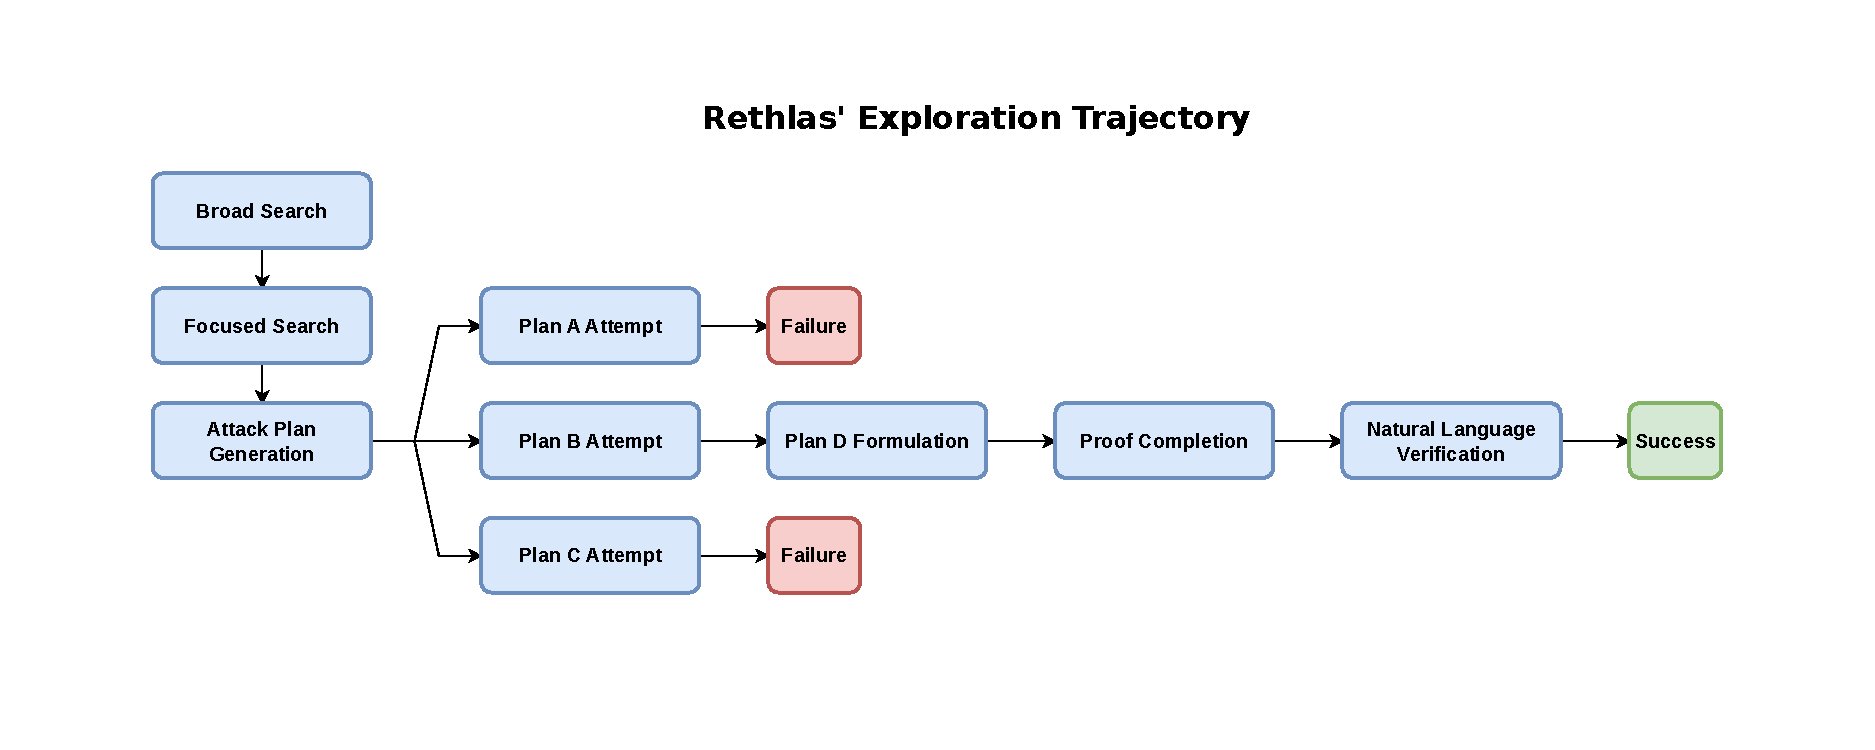
\includegraphics[width=\linewidth]{figure/rethlas_exploration_trajectory.pdf}
\caption{Rethlas 探索轨迹图示。}
\label{fig:rethlas_exploration}
\end{figure}

\begin{enumerate}[leftmargin=*]
    \item \textbf{广泛搜索。} 通过搜索最初的问题陈述及其参考文献，Rethlas 定位了将此问题记录为开放问题的文献，以及直接相关的技术资源，包括 \cite{cahen2014open, farley2016quasi}。这带来了一个更易于处理的重新表述：只需构造一个弱拟完备的环，它存在一个不是弱拟完备的同态象。
    \item \textbf{聚焦搜索。} 搜索上一步中重新表述的问题和相关结果，Rethlas 积累了进一步的技术理解。在此阶段，通过使用 Matlas 搜索查询 \verb`There exists a` \verb`weakly quasi-complete local ring with a quotient isomorphic to k[X,Y]_(X,Y).`，它发现了系统研究诺特局部环及其完备化之间关系（特别是关于一般形式纤维）的工作之一，即 \cite{fleming2019completely}。Rethlas 注意到，这一系列研究可能有助于构造所需的反例。
    \item \textbf{生成攻击计划。} 凭借从搜索结果中获得的知识，Rethlas 起草了三个分解计划来攻克这个问题。
    \begin{enumerate}[leftmargin=*]
        \item[A.] 构造一个弱拟完备环 \(R\)，它通过平方零扩张或理想化满射到一个已知的非弱拟完备局部环 \(S\)（理想情况下 \(S = k[X,Y]_{(X,Y)}\)）。
        \item[B.] 使用形式纤维控制构造一个弱拟完备局部整环 \(A\)，然后选择一个非素理想 \(I\)，使得商 \(A/I\) 的完备化表现出对弱拟完备性的明显阻碍。
        \item[C.] 从一个非弱拟完备的局部环 \(S\) 和一个具有极大理想 \(M\) 的弱拟完备扩环 \(T\) 开始。形成 \(T\) 的子环 \(R = S + M\) 或纤维积，并测试添加的 \(M\) 部分是否迫使 \(R\) 中具有零交集的每一个降链进入极大理想的幂。
    \end{enumerate}
    \item \textbf{尝试计划 A、B、C 并制定计划 D。} 计划 A 和 C 在几次尝试后失败，没有取得明显进展。在这些尝试中，继续研究将诺特局部环 \(A\) 与其完备化 \(T\) 联系起来的工作，使得 Jensen 的结果 \cite{jensen2006completions} 浮出水面。在此基础上，Rethlas 确定了一个具体的候选者 \(T = \mathbb{C}[[x,y,z]]/(x^2 - yz)\)，并提出了计划 D，它比计划 B 清晰得多。
    \begin{enumerate}[leftmargin=*]
        \item[D.] 使用 Jensen 的推论构造一个弱拟完备的局部 UFD \(A\)，其完备化 \(T\) 不是析因的，并且包含一个非主的高为一的素理想 \(Q\)；然后收缩 \(q = Q \cap A = (a)\) 产生一个不是弱拟完备的商 \(A/aA\)。
    \end{enumerate}
    \item \textbf{证明完成与验证。} Rethlas 算出了剩余的证明细节，并生成了一个 Markdown 文件，该文件清楚地陈述了所有引用的定理和论证的逻辑步骤。自然语言验证器接受了该证明，产生了最终输出。一些人类数学家认为可以忽略但形式化验证要求的一些次要细节并未完全填补；参见附录~\ref{subsubsec:gap-filling}。
\end{enumerate}

\section{形式化与验证}\label{sec:archon_results}

有了非形式证明在手，我们现在转向它在 Lean 4 中的形式化和验证。由 Archon 执行的形式化\footnote{完整的形式化代码开源在 \url{https://github.com/frenzymath/Anderson-Conjecture}。}，将 Anderson 猜想的完整证明翻译成了基于 Mathlib 的 Lean 4 项目，涵盖了主定理、所有支持性引理以及从六篇外部论文中提取的关键结果。这项任务绝非易事：除了常规的翻译之外，形式化还需要填补非形式论证中留下的隐含空白，以完整的细节实现未充分指定的构造（如超限递归），并调整证明策略以适应可用的库基础设施。根据对 Mathlib 贡献者的采访，我们估计一位经验丰富的形式化专家每天大约能产生 150-250 行 Lean 代码；因此，Archon 产生的 19,000 行代码库代表了相当于专家几个月工作量的工作负荷，在大约 80 小时的运行时间内自主完成。

我们首先对形式化输出及其关键的定量和定性特征进行概述（\Cref{subsec:overview-result}），然后讨论在此过程中吸取的经验教训和观察到的局限性（\Cref{subsec:lessons}）。

\toprule
\textbf{非形式组件} & \textbf{Lean 声明} & \textbf{文件} \\
\midrule
应用 Jensen 推论 2.4 & \texttt{jensen\_special\_case} & \texttt{Jensen/Jensen.lean} \\
平凡一般形式纤维 & \texttt{HasTrivialGenericFormalFiber} & \texttt{Jensen/Defs.lean} \\
\bottomrule
\end{tabular}
\end{center}

\subsection*{验证（条件 (A) 和 (B)）}

\begin{center}
\small
\begin{tabular}{p{5.5cm} l l}
\toprule
\textbf{非形式组件} & \textbf{Lean 声明} & \textbf{文件} \\
\midrule
$A$ 是 WQC（条件 (A)） & \texttt{a\_isWeaklyQuasiComplete} & \texttt{Main.lean} \\
$Q \ne (0)$ & \texttt{Q\_ne\_bot} & \texttt{Main.lean} \\
$q = Q \cap A$, $\operatorname{ht}(q) = 1$ & \texttt{contraction\_height\_one} & \texttt{Main.lean} \\
对于素元 $a$ 有 $q = (a)$（UFD） & \texttt{ufd\_height\_one\_principal} & \texttt{Main.lean} \\
$\dim(A/aA) = 1$ & \texttt{quotient\_prime\_dim\_one} & \texttt{Main.lean} \\
$A/aA$ 不是分析不可约的 & \texttt{quotient\_not\_analytically\_irreducible} & \texttt{Main.lean} \\
$\exists$ 不良商（条件 (B)） & \texttt{exists\_prime\_bad\_quotient} & \texttt{Main.lean} \\
\bottomrule
\end{tabular}
\end{center}

\subsection*{引用的文献结果}

非形式证明依赖于几个外部结果。我们描述了每一个结果是如何形式化的，以及相应的参考材料存储在何处（位于项目的 \texttt{references/} 目录中）。

\paragraph{Anderson (2014), \emph{Quasi-complete semilocal rings and modules}~\cite{anderson2014quasi}.}

证明中使用了本文的三个结果：
\begin{itemize}
\item \emph{Corollary~2.2}（一维局部整环：WQC $\Leftrightarrow$ 分析不可约）在 \texttt{QuasiCompleteRing/QuasiCompleteRing.lean} 中被形式化为 \texttt{dim1\_wqc\_iff\_analyticallyIrreducible}。
\item \emph{Theorem~5, Item~3}（QC $\Leftrightarrow$ 每个真商是 WQC）在 \texttt{QuasiCompleteRing/QuasiCompleteRing.lean} 中被形式化为 \texttt{isQuasiComplete\_iff\_quotients\_wqc}。
\item \emph{Theorem~3}（完备 $\Rightarrow$ 拟完备），最初归功于 Chevalley~\cite{chevalley1943theory}，按照 Anderson 的证明，在 \texttt{QuasiCompleteRing/Complete.lean} 中被形式化为 \texttt{anderson\_complete\_isQuasiComplete}。该结果出现在附录 A 的背景讨论中，但在主证明链中并不直接需要。
\end{itemize}
参考材料：\texttt{references/anderson\_2014.md}。

\paragraph{Farley (2016), \emph{Quasi-completeness and localizations of polynomial domains}~\cite{farley2016quasi}.}

Proposition~1（诺特局部整环是 WQC 当且仅当完备化的每个非零素理想与环非平凡相交）在 \texttt{QuasiCompleteRing/QuasiCompleteRing.lean} 中被形式化为 \texttt{isWeaklyQuasiComplete\_iff\_primes\_meet}。这个表征是建立条件~(A) 的关键工具。\\
参考材料：\texttt{references/farley\_2016.md}。

\paragraph{Jensen (2006), \emph{Completions of UFDs with Semi-Local Formal Fibers}~\cite{jensen2006completions}.}

Corollary~2.4（存在具有规定完备化和规定一般形式纤维的局部 UFD）在 \texttt{Jensen.lean} 中被形式化为 \texttt{jensen\_special\_case}，它将一般构造应用于特定的环~$T$。

基础构造（Jensen 的 Theorem~2.2，建立在 Heitmann~\cite{heitmann1993characterization} 和 Loepp~\cite{loepp1997constructing} 的基础上）是一个超限递归过程，它建立了一个 N-子环链，收敛到所需的 UFD。这是形式化中技术上最复杂的部分，跨越整个 \texttt{Jensen/} 子目录（约 15,000 行）。关键模块包括：
\begin{itemize}
\item \texttt{Jensen/Construction/}：主要的超限递归及其良基论证。
\item \texttt{Jensen/CloseUp/}：闭合过程，确保有限生成的理想在扩张下保持闭合。
\item \texttt{Jensen/KrullDomain/}：通过卡普兰斯基准则验证子环交集的 UFD 属性。
\item \texttt{Jensen/TransfiniteUnion.lean}：验证极限序数处的并集保留 N-子环属性。
\item \texttt{Jensen/Adjoin/}：添加超越元素同时保持代数不变量。
\item \texttt{Jensen/NSubring.lean}：N-子环和 A-扩张的定义。
\item \texttt{Jensen/Application.lean}：将一般构造应用于特定环~$T$。
\end{itemize}
参考材料：\texttt{references/jensen\_2006.md}, \texttt{references/heitmann\_1993.md}, \texttt{references/loepp\_1997.md}。

\paragraph{Chevalley (1943), \emph{On the theory of local rings}~\cite{chevalley1943theory}.}

Chevalley 关于完备蕴含拟完备的结果在 \texttt{QuasiCompleteRing/Complete.lean} 中被形式化为 \texttt{anderson\_complete\_isQuasiComplete}，遵循了 Anderson 推广（~\cite{anderson2014quasi} 的 Theorem~3）中给出的证明。\\
参考材料：\texttt{references/chevalley\_1943.md}。

\section{人类提供的证明蓝图}\label{appendix:human-blueprint}

本附录复制了在\Cref{subsubsec:ablation-human}描述的消融实验期间由人类主管提供给 Archon 的证明蓝图。该蓝图\emph{没有}在主要实验中使用。该文档以 Markdown 文件形式提供，并在此呈现，仅作了格式调整。它针对 Jensen 构造模块内部的 \texttt{UniqueFactorizationMonoid S\_sub} 的证明，提出了克鲁尔域方法作为 Archon 一直在追求的卡普兰斯基准则路线的替代方案。

\subsection*{数学背景}

设 $(T, M)$ 为完备诺特局部整环。设 $R$ 为 $T$ 的一个 N-子环（特别是 $R \subseteq T$ 的局部 UFD）。设 $y_1, y_2 \in R$ 是互素的，意义是没有 $R$ 的素元同时整除 $y_1$ 和 $y_2$。设 $x_1, x_2 \in T$ 在 $R$ 上是超越的，并且 $c = x_1 y_1 + x_2 y_2$，其中 $c \in R$。

定义：
\begin{itemize}
    \item $A_1 = R[x_1, y_2^{-1}]$,\quad $A_2 = R[x_2, y_1^{-1}]$
    \item $\tilde{R} = A_1 \cap A_2$
    \item $S_{\mathrm{sub}} = (\tilde{R} \cap (T \setminus M))^{-1}\tilde{R}$
\end{itemize}

\noindent\textbf{目标：} $S_{\mathrm{sub}}$ 是一个 UFD。

\subsection*{形式化建议}

应该定义一个环的 \texttt{IsKrullRing} 结构，意思是它（它的像）是其分式域中包含它的所有赋值子环的交集。这等价于：给定 $K$ 是 $R$ 的分式域，$R$ 的像是 $K$ 中包含它的所有赋值子环的交集。具有相同分式域的两个克鲁尔环的交集再次是一个克鲁尔环。

设 $d$ 为 $R$ 的一个元素，$K$ 为 $R$ 的分式域。应该将 $K$ 的赋值子环的一个属性定义为“由 $d$ 生成”，如果它包含 $R$ 并且它的极大理想由 $d$ 生成。在“分式域中由一个元素生成的赋值子环”（\texttt{ValuationSubring.IsPrincipalGen}）结构的定义中，这是 $R$ 的分式域的一个赋值子环的属性，要求它是一个 DVR，并且其极大理想由 $R$ 的某个素元 $d$ 的（像）生成。由素元 $d$ 生成的赋值子环自然是由元素生成的赋值子环。

此外，给定克鲁尔整环 $R$ 中的素元 $d$，需要具体构造 $K$ 的一个赋值子环，该子环正好是 $R$ 在由 $d$ 生成的素理想处的局部化。首先应构造此子环，证明（非平凡地，遵循本附录末尾的支持性引理）它是一个赋值子环，然后将其升级为赋值子环。

使用这些定义，可以更好地形式化该命题的以下证明。

\subsection*{证明}

\paragraph{第一步：化简到 $\tilde{R}$。} 因为 UFD 在任何乘法集处的局部化再次是 UFD，所以只需证明 $\tilde{R}$ 是 UFD。

\paragraph{第二步：$A_1$ 和 $A_2$ 是 UFD 也是克鲁尔整环。} 因为 $R$ 是 UFD 且 $x_1, x_2$ 在 $R$ 上是超越的，多项式环 $R[x_1]$ 和 $R[x_2]$ 是 UFD。分别在 $y_2$ 和 $y_1$ 处进行局部化保留了 UFD 属性，因此 $A_1$ 和 $A_2$ 是 UFD。每一个 UFD 都是一个克鲁尔整环：在由任何素元 $p$ 生成的素理想处的局部化是一个 DVR，UFD 是其分式域上所有这些 DVR 的交集，并且任何非零元素仅在有限多个这样的 DVR 中具有非零赋值。

\paragraph{第三步：$\tilde{R}$ 是一个克鲁尔整环。} 具有相同分式域的克鲁尔整环的有限交集再次是一个克鲁尔整环。$\tilde{R}$ 的本质 DVR 集合是通过取 $A_1$ 和 $A_2$ 的 DVR 族的并集获得的。有限性条件（任何元素仅在有限多个 DVR 中具有非零赋值）被继承。

\paragraph{第四步：$y_1 y_2$ 在 $\tilde{R}$ 中是素元的乘积。} 设 $p$ 是 $R$ 中 $y_1$ 的一个素因子。在 $A_1 = R[x_1, y_2^{-1}]$ 中，$p$ 仍然是素元，因为添加 $x_1$ 和对 $y_2$ 求逆（与 $y_1$ 互素）不影响 $p$。在 $A_2 = R[x_2, y_1^{-1}]$ 中，$p$ 变成一个单位，因为 $p \mid y_1$ 且 $y_1$ 被求逆。因此，在克鲁尔整环 $\tilde{R}$ 中，$p$ 的赋值分布在恰好一个 DVR（来自 $A_1$ 一侧）处为 $1$，在其他任何地方都为 $0$。具有这种分布的元素不能被进一步分解，所以 $p$ 在 $\tilde{R}$ 中是素元。同样的论证对称地适用于 $y_2$ 的素因子。

\paragraph{第五步：$\tilde{R}[(y_1 y_2)^{-1}]$ 是一个 UFD。} 我们计算：
\[
\tilde{R}[(y_1 y_2)^{-1}] = A_1[y_1^{-1}] \cap A_2[y_2^{-1}] = R[x_1, y_1^{-1}, y_2^{-1}] \cap R[x_2, y_1^{-1}, y_2^{-1}].
\]
关系式 $c = x_1 y_1 + x_2 y_2$ 意味着 $x_2 = (c - x_1 y_1)/y_2$，所以 $R[x_1, y_1^{-1}, y_2^{-1}] = R[x_2, y_1^{-1}, y_2^{-1}]$，因此
\[
\tilde{R}[(y_1 y_2)^{-1}] = R[x_1, (y_1 y_2)^{-1}],
\]
这是多项式 UFD $R[x_1]$ 的一个局部化，因此是一个 UFD。

\paragraph{第六步：应用 Nagata 引理。} 我们现在剩下了一个经典的设置（Nagata 定理的一个变体）：$\tilde{R}$ 是一个克鲁尔整环，$y = y_1 y_2$ 在 $\tilde{R}$ 中是素元的乘积，且 $\tilde{R}[y^{-1}]$ 是一个 UFD。我们必须证明 $\tilde{R}$ 是一个 UFD。为此，我们只需要证明对于 $\tilde{R}$ 中的任何元素，素因式分解的存在性和唯一性。

\emph{分解的存在性。} 取 $\tilde{R}$ 中任意的非零非单位元素 $a$。因为 $\tilde{R}[y^{-1}]$ 是 UFD，我们可以在局部化环中对 $a$ 进行因式分解。为了将这种分解拉回 $\tilde{R}$，我们调整 $y$ 的素因子的幂。由于 $\tilde{R}$ 是一个克鲁尔整环，$a$ 在对应于 $y$ 的素因子的 DVR 处的赋值是严格有限的（这防止了提取 $y$ 的无限次幂的病态情况）。我们可以完美地从 $a$ 中提取出这些 $y$-素元的精确有限次幂，留下一个元素 $a'$，其在 $\tilde{R}[y^{-1}]$ 中的素因式分解完全由与 $y$ 互素的素元组成。我们乘以适当的 $y$ 的幂以清除分母，使得这种因式分解完全位于 $\tilde{R}$ 中。

\emph{拉回因子的素性。} 我们必须验证这些拉回的因子（让我们称其中任意一个为 $q$）在基环 $\tilde{R}$ 中仍然是素元。假设为了寻求矛盾，$q$ 在 $\tilde{R}$ 中不是素元。因为 $q$ 映射到 $\tilde{R}[y^{-1}]$ 中的一个素元，它在局部化环中的赋值分布有恰好一个非零条目（即 $1$）。如果 $q$ 在 $\tilde{R}$ 中分解，它在 $\tilde{R}$ 的 DVR 上的赋值分布必须分裂，这意味着 $q$ 将在两个或更多 DVR 处具有 ${>}\,0$ 的赋值，或者在单个 DVR 处具有 ${>}\,1$ 的赋值。然而，局部化 $\tilde{R}[y^{-1}]$ 的 DVR 集合正好是 $\tilde{R}$ 的 DVR 集合减去对应于 $y$ 的素因子的那些。因为我们特意调整了 $q$ 使得其在 $y$-DVR 处的赋值为 $0$，所以 $q$ 在 $\tilde{R}$ 中的赋值分布与其在 $\tilde{R}[y^{-1}]$ 中的赋值分布相同：恰好在一个 DVR 处为 $1$，在其他任何地方都为 $0$。一个在单个 DVR 处 $v(q) = 1$ 且在别处为 $0$ 的元素不能被进一步分解。因此，$q$ 在 $\tilde{R}$ 中是素元。

\paragraph{第七步：结论。} 因为 $\tilde{R}$ 中的任何元素都可以被分解为素元，所以 $\tilde{R}$ 是一个 UFD。最后，因为 $S_{\mathrm{sub}}$ 是 $\tilde{R}$ 在乘法集 $\tilde{R} \cap (T \setminus M)$ 处的局部化，并且 UFD 的局部化始终是 UFD，我们得出结论 $S_{\mathrm{sub}}$ 是一个 UFD。

\subsection*{支持性引理：在克鲁尔整环中素元处的局部化}

\noindent\textbf{引理。} \textit{设 $A$ 为一个克鲁尔整环，设 $t \in A$ 为一个素元。那么在素理想 $(t)$ 处的局部化 $A_{(t)}$ 是一个 DVR。}

\begin{proof}
设 $P = (t)$。局部化环 $A_P$ 是一个具有极大理想 $tA_P$ 的局部整环。我们展示在 $A$ 中 $\bigcap_{n=1}^{\infty} (t^n) = (0)$。为了寻求矛盾，假设一个非零 $x \in A$ 对于所有 $n \geq 1$ 满足 $x = a_n t^n$。根据克鲁尔整环的定义，$A$ 与其分式域上的一族离散赋值 $\{v_i\}_{i \in I}$ 相关联，使得 $A = \{a \in K \mid \text{对于所有 } i, v_i(a) \geq 0\}$，并且对于任何非零元素，只有有限多个 $v_i$ 取正值。选择一个满足 $v(t) \geq 1$ 的赋值 $v$。那么对于每一个 $n \geq 1$，都有 $v(x) = v(a_n) + n \cdot v(t) \geq n$，这迫使 $v(x) = \infty$，与 $x \neq 0$ 矛盾。由于 $A_P$ 是一个具有主极大理想且 $\bigcap_{n=1}^{\infty} (tA_P)^n = (0)$ 的局部整环，它是一个 DVR。
\end{proof}


\section{形式化中的详细数学示例}\label{appendix:detailed-examples}

本附录提供了在\Cref{subsec:lessons}中讨论的值得注意的行为的详细数学描述。每个小节对应一个具体的观察结果，并包含理解它所必需的数学背景。

\subsection{在证明细节中自动填补空白}\label{subsubsec:gap-filling}

Archon 展示了自主提供非形式证明所省略的非平凡数学论证的能力。我们用两个例子来说明。

非形式证明断言
\[
T = \mathbb{C}[[x,y,z]]/(x^2 - yz)
\]
通过 $x \mapsto uv$, $y \mapsto u^2$, $z \mapsto v^2$ 同构于子环 $\mathbb{C}[[u^2, uv, v^2]] \subseteq \mathbb{C}[[u,v]]$。虽然这些分配很容易定义到子环上的满射，但建立单射性需要一个单独的论证，而非形式证明没有提供。Archon 通过在幂级数系数层面上明确构造一个商函数并逐项验证核中的每一个元素都能被生成元 $x^2 - yz$ 整除，从而解决了这个问题，从而在不查阅任何外部参考资料的情况下完成了单射性证明。

第二个例子涉及基数等式 $|T| = |T/\mathfrak{m}| = |\mathbb{C}|$，非形式证明只是陈述了这一点而没有详细说明。这个等式并非微不足道：对于幂级数环 $k[[x_1, \ldots, x_n]]$，有 $|k[[x_1, \ldots, x_n]]| = |k|^{\aleph_0}$，并且对于一般无限基数 $\kappa$，$\kappa^{\aleph_0} = \kappa$ 并\emph{不}成立。Archon 正确地识别出该等式依赖于连续统 $\mathfrak{c} = 2^{\aleph_0}$ 的特殊性质，即 $\mathfrak{c}^{\aleph_0} = (2^{\aleph_0})^{\aleph_0} = 2^{\aleph_0 \cdot \aleph_0} = 2^{\aleph_0} = \mathfrak{c}$，并应用相应的 Mathlib 引理填补了这一空白。

\subsection{处理未充分指定的超限构造}\label{subsubsec:transfinite}

构造具有规定完备化的局部 UFD $A$ 依赖于 Jensen~\cite{jensen2006completions} 的超限递归程序，该程序建立在 Loepp~\cite{loepp1997constructing} 和 Heitmann~\cite{heitmann1993characterization} 的早期工作之上。源论文在很高层次上描述了这一构造——指出应该“递归地定义 $\{R_\alpha\}_{\alpha \in V}$”并“在极限序数处取并集”——但把簿记细节留给了读者。在 Lean 4 中形式化这样的构造要求使递归的每一个方面都变得明确：在每一步携带的数据、良基论证、代数不变量通过后继和极限阶段的传播，以及每一级精确的基数界限。

Archon 通过设计一个捆绑记录类型解决了这一挑战，该类型将递归的每个阶段连同其前驱、扩张关系、基数界限和闭包属性打包在一起。它通过对序数的良基递归实现了递归，并在每一级显式跟踪界限 $\max(\aleph_0, |\{\gamma \le \alpha\}|)$。极限序数的情况通过一个专门的模块处理，该模块验证 N-子环链的并集保留了 UFD 属性、素扩张条件和基数约束。实际上，Archon 成功地将一个庞大的超限论证分解为模块化、可独立验证的代数组件——将所有技术交换代数步骤从归纳支架中分离出来——然后将它们组装成一个完整的形式化证明。达到这个最终架构本身就是一个非平凡的过程：Archon 的初步尝试依赖于一种不正确的证明策略，它通过跨越多个会话的大规模重构诊断并纠正了该策略（附录~\ref{subsubsec:self-diagnosis}和~\ref{subsubsec:refactoring}）。

\subsection{数学错误的自我诊断}\label{subsubsec:self-diagnosis}

在对超限构造的最初尝试中，Archon 采用了佐恩引理（Zorn's lemma）来产生一个极大元，而不是执行证明所需的显式超限递归。此外，它将“基数严格小于连续统”与“可数”混为一谈——这种等同在连续统假设下是有效的，但在仅凭 ZFC 的情况下是无法证明的。这些错误导致了下游的代数步骤失败：无法建立必要的基数界限，并且在极限阶段所需的闭包属性不成立。

值得注意的是，源论文并没有明确警告这些陷阱。Archon 通过其自身的诊断过程找出了失败的根本原因：它认识到佐恩引理只产生存在性，而没有构造所需的对中间阶段的细粒度控制，并且在没有连续统假设的情况下，可数性假设是不合理的。这种自我诊断是在没有人类指导的情况下进行的，并直接导致了下面描述的正确重构。

\subsection{跨会话架构重构}\label{subsubsec:refactoring}

在认识到附录~\ref{subsubsec:self-diagnosis}中描述的错误后，Archon 对超限构造进行了大规模重构，用显式的良基递归取代了基于佐恩引理的方法，并修改了所有基数论证，使用一般基数算术代替可数性假设。这种重构跨越了多个智能体会话——要求智能体在上下文边界保持对整体证明架构的连贯理解——并涉及在整个 Jensen 构造模块中重组相互依赖的文件。

\subsection{替代证明策略的发现}\label{subsubsec:alternative-strategy}

构造中的一个关键技术引理——对应于 Heitmann~\cite{heitmann1993characterization} 的 Lemma 4——建立了一个特定子环的交集是 UFD。原始证明的进行方式是，证明该交集是一个克鲁尔整环，然后诉诸于高为一的素理想的分类。然而，Mathlib 目前并未提供克鲁尔整环的形式化定义，忠实地遵循原始论证将要求 Archon 开发大量额外的基础设施，包括克鲁尔整环的刻画和除子理想理论。

相反，Archon 独立地识别并应用了卡普兰斯基准则（Kaplansky's criterion）——它将 UFD 刻画为每一个非零素理想都包含一个素元的整环——直接建立了该结果。这条没有出现在提供给智能体的任何参考论文中的替代路线，完全绕过了对克鲁尔整环理论的需求，并产生了一个更简洁的形式化。这段经历说明了 Archon 有能力根据可用的库支持调整其证明策略，而不是僵化地遵循非形式论证的结构。


\section{通过 Comparator 的陈述验证}\label{appendix:szm_comparator}

正如在\Cref{subsec:overview-result}中所述，我们在两个层面上验证形式化的正确性。首先，整个项目通过了 \texttt{lake build}，证实所有证明义务都被履行。其次，我们使用 Comparator~\cite{comparator} 确认完整项目中证明的定理与一个简短、人类可读的规范相匹配，并且仅依赖于标准的 Lean 公理。

规范文件 \texttt{Challenge.lean} 复制如下。它仅包含拟完备和弱拟完备的定义，以及主定理的陈述。人类评审者可以验证这 30 行代码的语义正确性，而无需了解证明或代码库的其余部分。然后，Comparator 会自动检查完整项目中的 \texttt{main\_theorem} 声明是否完全证明了这一陈述，且没有隐藏的公理。

\begin{Verbatim}[fontsize=\small,commandchars=!?\|]
import Mathlib.Algebra.Algebra.Operations
import Mathlib.RingTheory.LocalRing.MaximalIdeal.Defs
import Mathlib.RingTheory.Noetherian.Defs

variable (R : Type*) [CommRing R] [IsLocalRing R]

/-- A local ring `R` is quasi-complete if for any antitone sequence
of ideals `A : !(!mathbb?N|!) → Ideal R` and each `k : !(!mathbb?N|!)`, there exists `s`
such that `A s !(!le!) (!(!sqcap!) n, A n) !(!sqcup!) (IsLocalRing.maximalIdeal R) ^ k`.

This is Definition 1.1 of Anderson (2014). -/
def IsQuasiComplete : Prop :=
  !(!forall!) (A : !(!mathbb?N|!) → Ideal R), Antitone A →
    !(!forall!) (k : !(!mathbb?N|!)), !(!exists!) s,
      A s !(!le!) (!(!sqcap!) n, A n) !(!sqcup!) (IsLocalRing.maximalIdeal R) ^ k

/-- A local ring `R` is weakly quasi-complete if for any antitone
sequence of ideals `A : !(!mathbb?N|!) → Ideal R` with `!(!sqcap!) n, A n = !(!bot!)` and
each `k : !(!mathbb?N|!)`, there exists `s` such that
`A s !(!le!) (IsLocalRing.maximalIdeal R) ^ k`. -/
def IsWeaklyQuasiComplete : Prop :=
  !(!forall!) (A : !(!mathbb?N|!) → Ideal R), Antitone A → (!(!sqcap!) n, A n) = !(!bot!) →
    !(!forall!) (k : !(!mathbb?N|!)), !(!exists!) s,
      A s !(!le!) (IsLocalRing.maximalIdeal R) ^ k

/-- **Main Theorem**: There exists a weakly quasi-complete
Noetherian local ring that is not quasi-complete. -/
theorem main_theorem :
    !(!exists!) (R : Type) (_ : CommRing R) (_ : IsLocalRing R)
      (_ : IsNoetherianRing R),
      IsWeaklyQuasiComplete R !(!wedge!) ¬ IsQuasiComplete R := by
  sorry
\end{Verbatim}
\noindent 此文件中的 \texttt{sorry} 是有意为之的：它标记了完整项目必须履行的一项义务。Comparator 会验证项目的 \texttt{main\_theorem} 是否以完整的证明填补了这个 \texttt{sorry}，并与陈述完全匹配。
\let\clearpage\relax
\end{document}
